\documentclass[ 11pt, oneside, italian, onehalfspacing, headsepline, ]{MastersDoctoralThesis}

\usepackage[utf8]{inputenc} % Required for inputting international characters
\usepackage[T1]{fontenc} % Output font encoding for international characters
%\usepackage{mathpazo} % Use the Palatino font by default
\usepackage[backend=bibtex, sorting=none, natbib=true]{biblatex} % Use the bibtex backend with the authoryear citation style (which resembles APA)
\usepackage[autostyle=true]{csquotes} % Required to generate language-dependent quotes in the bibliography
\usepackage{enumitem}
\usepackage{listings}
\usepackage{graphicx}
\usepackage{xcolor}
\usepackage{amsmath}
\usepackage[font={small}]{caption}
\usepackage{varwidth}
\usepackage{supertabular}
\usepackage[caption=false]{subfig}
\usepackage{wrapfig}
\usepackage{mathtools}
\usepackage{titlesec}
\usepackage{hyperref}

\newcommand\citen[1]{\citeauthor{#1} \citep{#1}}
\newcommand\citetitlen[1]{\citetitle{#1} \citep{#1}}
\addbibresource{related_work.bib} % The filename of the bibliography

\graphicspath{
    {Figures/}{images/}
}

\newenvironment{blueparagraph}{\par\color{blue}}{\par}
\newenvironment{nscenter}
 {\parskip=0pt\par\nopagebreak\centering}
 {\par\noindent\ignorespacesafterend}

 \titleformat{\chapter}[display]
 {\normalfont\bfseries}{}{0pt}{\huge}

%----------------------------------------------------------------------------------------
%	MARGIN SETTINGS
%----------------------------------------------------------------------------------------

\geometry{
	paper=a4paper, % Change to letterpaper for US letter
	inner=2.5cm, % Inner margin
	outer=3.8cm, % Outer margin
	bindingoffset=.5cm, % Binding offset
	top=1.5cm, % Top margin
	bottom=1.5cm, % Bottom margin
	%showframe, % Uncomment to show how the type block is set on the page
}

\usepackage{graphicx}
\usepackage{multicol}

\setlength{\columnsep}{0.3in}

\pdfpagewidth 8.5in
\pdfpageheight 11in

\setlength{\textwidth}{6.5in}
\setlength{\oddsidemargin}{0.0in}
\setlength{\evensidemargin}{0.0in}
\setlength{\textheight}{9in}
\setlength{\topmargin}{-36pt}
\setlength{\headheight}{12pt}
\setlength{\headsep}{24pt}
\setlength{\footskip}{24pt}
\setlength{\parskip}{4pt plus 1pt}
\renewcommand{\baselinestretch}{1.125} %1.0

\pagenumbering{arabic}

%   PUNCTUATION SPACING
%  By default, punctuation [.?!:;,] is followed by extra space EXCEPT
%  when the punctuation follows an upper case letter.  The following
%  removes the exception, i.e., punctuation will produce extra space
%  regardless of what character precedes the punctuation.  If you
%  don't want the extra space, follow the offending punctuation mark
%  with '\ ' or '~'.  \frenchspacing and \nonfrenchspacing work as
%  usual to turn extra spacing off and back on, respectively.

\sfcode`A=1000 \sfcode`B=1000 \sfcode`C=1000 \sfcode`D=1000
\sfcode`E=1000 \sfcode`F=1000 \sfcode`G=1000 \sfcode`H=1000
\sfcode`I=1000 \sfcode`J=1000 \sfcode`K=1000 \sfcode`L=1000
\sfcode`M=1000 \sfcode`N=1000 \sfcode`O=1000 \sfcode`P=1000
\sfcode`Q=1000 \sfcode`R=1000 \sfcode`S=1000 \sfcode`T=1000
\sfcode`U=1000 \sfcode`V=1000 \sfcode`W=1000 \sfcode`X=1000
\sfcode`Y=1000 \sfcode`Z=100


%----------------------------------------------------------------------------------------
%	THESIS INFORMATION
%----------------------------------------------------------------------------------------

\thesistitle{Identificazione Estensioni Malevove di Firefox} % Your thesis title, this is used in the title and abstract, print it elsewhere with \ttitle

\author{Daniele \textsc{Albanese}} % Your name, this is used in the title page and abstract, print it elsewhere with \authorname


\subject{Networking security and software security} % Your subject area, this is not currently used anywhere in the template, print it elsewhere with \subjectname
\keywords{Browser, extension, malicious} % Keywords for your thesis, this is not currently used anywhere in the template, print it elsewhere with \keywordnames
\university{\href{https://www.unimol.it/}{Università del Molise}} % Your university's name and URL, this is used in the title page and abstract, print it elsewhere with \univname
\department{\href{http://dipbioter.unimol.it/}{Dipartimento di Bioscienze e Territorio}} % Your department's name and URL, this is used in the title page and abstract, print it elsewhere with \deptname3

\AtBeginDocument{
\hypersetup{pdftitle=Title\ttitle} % Set the PDF's title to your title
\hypersetup{pdfauthor=Daniele Albanese\authorname} % Set the PDF's author to your name
\hypersetup{pdfkeywords=keyword1 keyword2 keyword3 \keywordnames} % Set the PDF's keywords to your keywords
}

\begin{document}
\renewenvironment{abstract}


\pagestyle{plain} % Default to the plain heading style until the thesis style is called for the body content

%----------------------------------------------------------------------------------------
%	TITLE PAGE
%----------------------------------------------------------------------------------------

\begin{titlepage}
	\begin{center}
				
		\vspace*{.06\textheight}
		{\scshape\LARGE \univname\par}\vspace{0.5cm} % University name
		{\scshape\large \deptname\par}\vspace{1cm} % University name
				
		
\includegraphics[width=0.25\textwidth]{images/logo.png} % University/department logo - uncomment to place it
		\vspace{1cm}
				
		\textsc{\Large Proposta di progetto}\\[0.5cm] % Thesis type
				
		\HRule\\[0.4cm] % Horizontal line
		{\huge \bfseries \ttitle\par}\vspace{0.4cm} % Thesis title
		\HRule\\[1.5cm] % Horizontal line
				
				
		\begin{center} \large
			\emph{Author:}\\
			\href{mailto:d.albanese1@studenti.unimol.it}{\authorname} % Author name - remove the \href bracket to remove the link
		\end{center}
				
		\centerline{\large \subjectname}
				
		{\large Dicembre 10, 2020}\\[2cm] % Date
		\vfill
	\end{center}
\end{titlepage}

%----------------------------------------------------------------------------------------
%	PROPOSAL
%----------------------------------------------------------------------------------------

{\chapter{Introduzione}}

Poiché gli utenti soddisfano sempre più le loro esigenze informatiche attraverso il \textit{Web}, i \textit{browser Web} moderni, devono fornire maggiori funzionalità e personalizzazione. \newline 
Una caratteristica indispensabile dei \textit{browser} moderni è la possibilità di essere personalizzati, lato client, tramite delle \textit{estensioni}. \newline
Utilizzando le \textit{estensioni}, gli utenti possono aumentare e modificare il comportamento dei loro browser per soddisfare le loro esigenze. \newline
Una delle possibili esigenze degli utenti, per cui vengono utilizzate le \textit{estensioni}, è quella di aumentare la propria produttività come, ad esempio: bloccando gli annunci e/o i tracciamenti indesiderati o offrendo nuovi modi per organizzare schede e segnalibri. \newline
Dato l'aumento delle \textit{estensioni} una volta benigne divenute maligne, nell'articolo preso in esame \citep{ReferenceArticle}, viene proposto un nuovo metodo per il rilevamento delle \textit{estensioni dannose} del \textit{browser}, concentrandosi sui loro delta di aggiornamento. \par
Data un'estensione diventata \textit{dannosa}, il loro sistema utilizza l'ultima versione benigna di tale estensione, per identificare il codice responsabile delle sue azioni \textit{malevole}. Concentrandosi sulle API abusate da questo codice-delta, il sistema crea una sequenza di API, che verrà ricercata in tutte le altre estensioni presenti all'interno dello Store. \newline
In questo modo, il sistema utilizza le estensioni dannose precedentemente trovate e le categorizza come estensioni  \textit{''seme''}, che verrano poi utilizzate per identificare estensioni con aggiornamenti simili, quindi, che utilizzano API potenzialmente dannose, che non sono state ancora rilevate dal sistema o contrassegnate dagli utenti.

\begin{figure}[hbt!]
	\caption{Data sources collection and workflow of malicious extension detection pipeline. Analysus from User Feedback (\textbf{1}) and malisious JavaScript clustering (\textbf{2}) from seed extensions}\label{fig:summarydiagram}
	\centering
	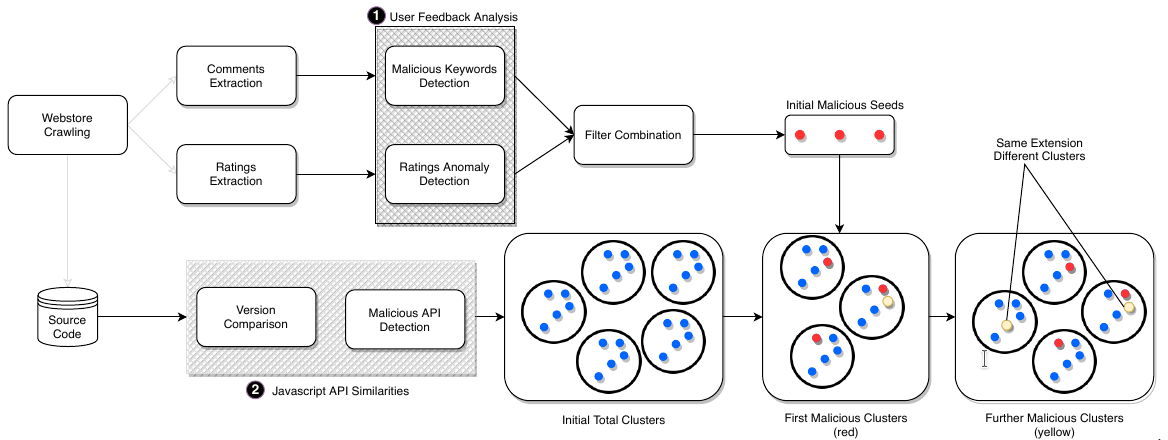
\includegraphics[width=0.8\textwidth]{Summary_diagram.png}
\end{figure}

\par

Fatta questa premessa, andremo ora ad analizzare, come verrà rapportato, il sistema descritto in precedenza, avendo come browser di analisi, non più il browser \textbf{Google Chrome}, ma il browser \textbf{Mozilla Firefox}. \newline

Il \textit{browser Firefox} utilizza \textbf{Firefox Browser ADD-ONS} \citep{FirefoxAddOnsStore} come repository ufficiale per la pubblicazione e la distribuzione delle estensioni agli utenti. 

{\section{Codice sorgente}}

Le estensioni sono distribuite nel negozio sotto forsa di file \textit{.xpi} ovvero, un semplice archivio ZIP con un'estensione speciale. All'interno di questo file \textbf{XPI} risiedono tutti i file dell'estensione ovvero, il \textit{codice sorgente} (JavaScript, HTML e CSS), le \textit{immagini locali}, ed un file \textit{manifest.json}. In questo file \textit{manifest.json}, sono contenuti tutti i metadati dell'estensione in formato \textbf{JSON}, nello specifico, è presente il nome, la versione, la descrizione dell'estensione, nonché le autorizzazioni richieste. \newline

Le due principali categorie di script presenti all'interno delle estensioni sono: i \textit{background script} ed i \textit{content script}. Il primo  è uno script eseguito durante l'attività dell'estensione, responsabile della maggior parte delle funzionalità in backgorund. Possono esserci più \textit{background script} ma, nella maggior parte delle estensioni, ne è presente soltanto uno. Il secondo tipo invece, è un file \textbf{JS} in esecuzione nel contesto della pagina web visitata e che utilizza i \textbf{DOM} (\textbf{D}ocument \textbf{O}bject\textbf{M}odel) per modificare le pagine web. Per questo tipo di scritp, né è presente più di uno. Oltre queste due principali categorie di script, potrebbe essere presente del codice \textbf{JS} di supporto, come, ad esempio, librerie di terze parti.

{\section{Commenti e voti}}

Oltre a raccogliere il codice sorgente delle estensioni, il sistesta raccoglierà altri dati disponibili sullo \textbf{Store}. Per ogni estensione attiva sullo \textbf{Store}, verrà eseguita una scansione di tutte le informazioni disponibili nella sua pagine, compreso il numero totale di valutazioni, la valutazione media totale, i download totali e l'autore dell'estensione. Inoltre, verranno raccolti tutti i commenti che, gli utenti hanno scritto per ciascuna estensione e per ogni commento verrà raccolta la \textit{valutazione}, il  \textit{giorno di pubblicazione} ed il  \textit{nome dell'autore}.

{\chapter{Metodologia}}

Il sitema di analisi delle estensioni consisterà in due fasi principali: utilizzare i feedback degli utenti e, raggruppare il codice sorgente delle estesioni in base alle API JavaScript.

{\section{Fase 1}}

La logica di questa prima fase è basata sui feedback degli utenti esperti, che osservano un'estensione precedentemente  \textit{benigna}, comportarsi in modo  \textit{malizioso} e, non solo la disinstalleranno, ma almeno alcuni di loro, lasceranno un feedback negativo attraverso il sistema di recensioni. Questo feedback avrà lo scopo di allarme per altri utenti che potrebbero prendere in considerazione l'installazione dell'estensione in questione. \par

Per identificare quanti commenti saranno necessari per identificare le anomalie di rating, verranno eseguiti una serie di esperimenti utilizzando il pacchetto statico \textit{Anomalize} \citep{Anomalize}. \textit{Anomalize} può essere utilizzato per identificare tendenze e componenti stagionali in serie temporali \citep{GeneralizedExtremeStudentized}. Come le tipiche tecniche di rilevamento delle anomalie, questo processo comprende due fasi, la \textit{fase di addestramento} e la \textit{fase di test/rilevalento}. Nella \textit{fase di addestramento}, verrà utilizzata la parte iniziale della sequenza di valutazioni, per impostare una verità di base per le valutazioni tipiche, che una data estensione riceve. Quindi verrà utilizzato il resto dei dati per trovare anomalie nelle valutazioni.

{\section{Fase 2}}

Nella \textit{fase 2}, verranno utilizzate le estensioni contrassegnate come dannose dalla \textit{fase 1}, e verrà identificato l'aggiornamento del codice, che corrisponde all'estensione che passa da benigna a maligna. Verà codificato questo aggiornamento  in termini di API critiche, e verrà cercato per altre estensioni con aggiornamenti simili. Attraverso questo processo, verranno identificate altre estensioni, che mostrano segni simili di aggiornamenti dannosi, ma che ancora non sono state contrassegnate, né dagli utenti né dallo \textbf{Store}.

{\chapter{Delivery}}

Per quanto riguarda la fase di \textit{''Delivery''} verrà prodotto un documento con i risultati dello studio e tutto il codice sarà disponibile sulla piattaforma \href{https://github.com/dj-d/FoxWall}{GitHub}.

%----------------------------------------------------------------------------------------

\printbibliography\
\end{document}
